
\subsection{Aerodynamic Data Design}
\label{sec:aerodynamic-databases}

\subsubsection{Reference Geometry and Airfoil Parameterization}
\label{sec:reference-geometry}

A transonic clean-wing configuration adopted from previous work is used as reference geometry to provide a consistent geometric basis for the aerodynamic data. The reference half-wing has a straight-tapered planform with a root chord of \SI{5.0}{m}, a tip chord of \SI{1.5}{m}, and a semispan of \SI{14.0}{m}. The leading-edge and quarter-chord sweep angles are $28.18^\circ$ and $25.32^\circ$, respectively, as shown in Fig.~\ref{fig:reference-wing-planform}. Six baseline airfoil sections are extracted at the normalized spanwise locations $\eta=0.0$, $0.2$, $0.4$, $0.6$, $0.8$, and $1.0$, with their geometries shown in Fig.~\ref{fig:reference-airfoil-sections}. These sections preserve the spanwise variations in airfoil shape and thickness and provide a common geometric origin for the aerodynamic data.

\begin{figure}[!htb]
    \centering
    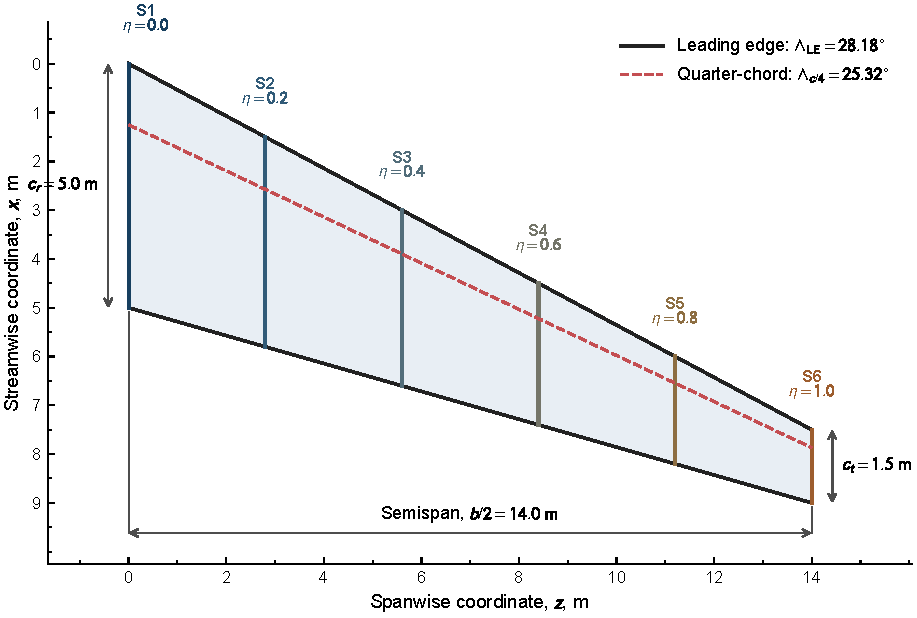
\includegraphics[width=0.84\linewidth]{II_Database_and_Preprocessing/figures/II_A_Fig01/II_A_Fig01_reference_wing_planform.pdf}
    \caption{Reference half-wing planform, principal dimensions, and spanwise locations of the six baseline airfoil sections, where $\eta=2z/b$ denotes the normalized semispan coordinate.}
    \label{fig:reference-wing-planform}
\end{figure}

\begin{figure}[!htb]
    \centering
    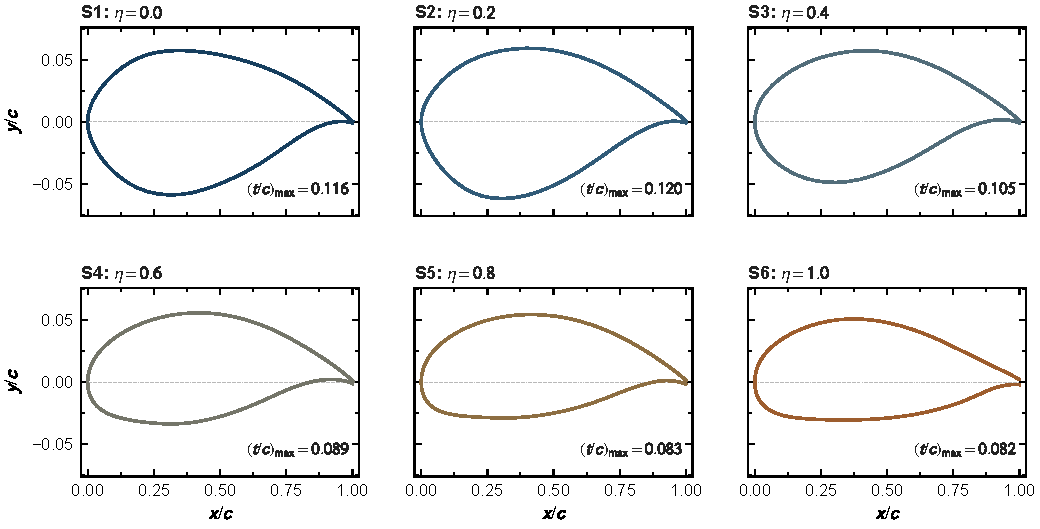
\includegraphics[width=0.98\linewidth]{II_Database_and_Preprocessing/figures/II_A_Fig02/II_A_Fig02_reference_airfoil_sections.pdf}
    \caption{Baseline airfoil profiles extracted at six spanwise stations of the reference wing and expressed in local chord-normalized coordinates.}
    \label{fig:reference-airfoil-sections}
\end{figure}

To introduce continuous shape variations while retaining the characteristics of the baseline profiles, the class--shape transformation (CST) method \cite{Kulfan2008} is employed to parameterize each airfoil section. For the upper and lower surfaces $s\in\{u,l\}$, the geometry is expressed as
\[
    \frac{y_s(\xi)}{c}
    = \xi^{1/2}(1-\xi)
      \sum_{i=0}^{4} A_{i,s}\binom{4}{i}\xi^i(1-\xi)^{4-i}
      + \xi t_s,
    \qquad \xi=\frac{x}{c},
\]
where $A_{i,s}$ denotes the corresponding Bernstein-polynomial shape coefficient and $t_s$ is the derived nondimensional trailing-edge ordinate of surface $s$. Each sampled airfoil is generated by perturbing the CST coefficients of its respective baseline section rather than by scaling a single reference airfoil. This treatment retains the differences among the spanwise sections while allowing their shapes to vary parametrically.


\subsubsection{Knowledge-Domain Databases}
\label{sec:database-architecture}
\label{sec:design-space}

The surface-pressure distribution of a finite wing reflects both the sectional aerodynamic response associated with local airfoil geometry and flow conditions and the additional three-dimensional effects of finite span, which are particularly pronounced near the wing root and tip. To characterize these contributions separately, two knowledge-domain databases are constructed using infinite-span swept wings and constant-chord finite-span wings. Their geometric and operating-condition correspondence enables the extraction of finite-span pressure corrections, as illustrated in Fig.~\ref{fig:database-architecture}.


\begin{figure}[!htb]
    \centering
    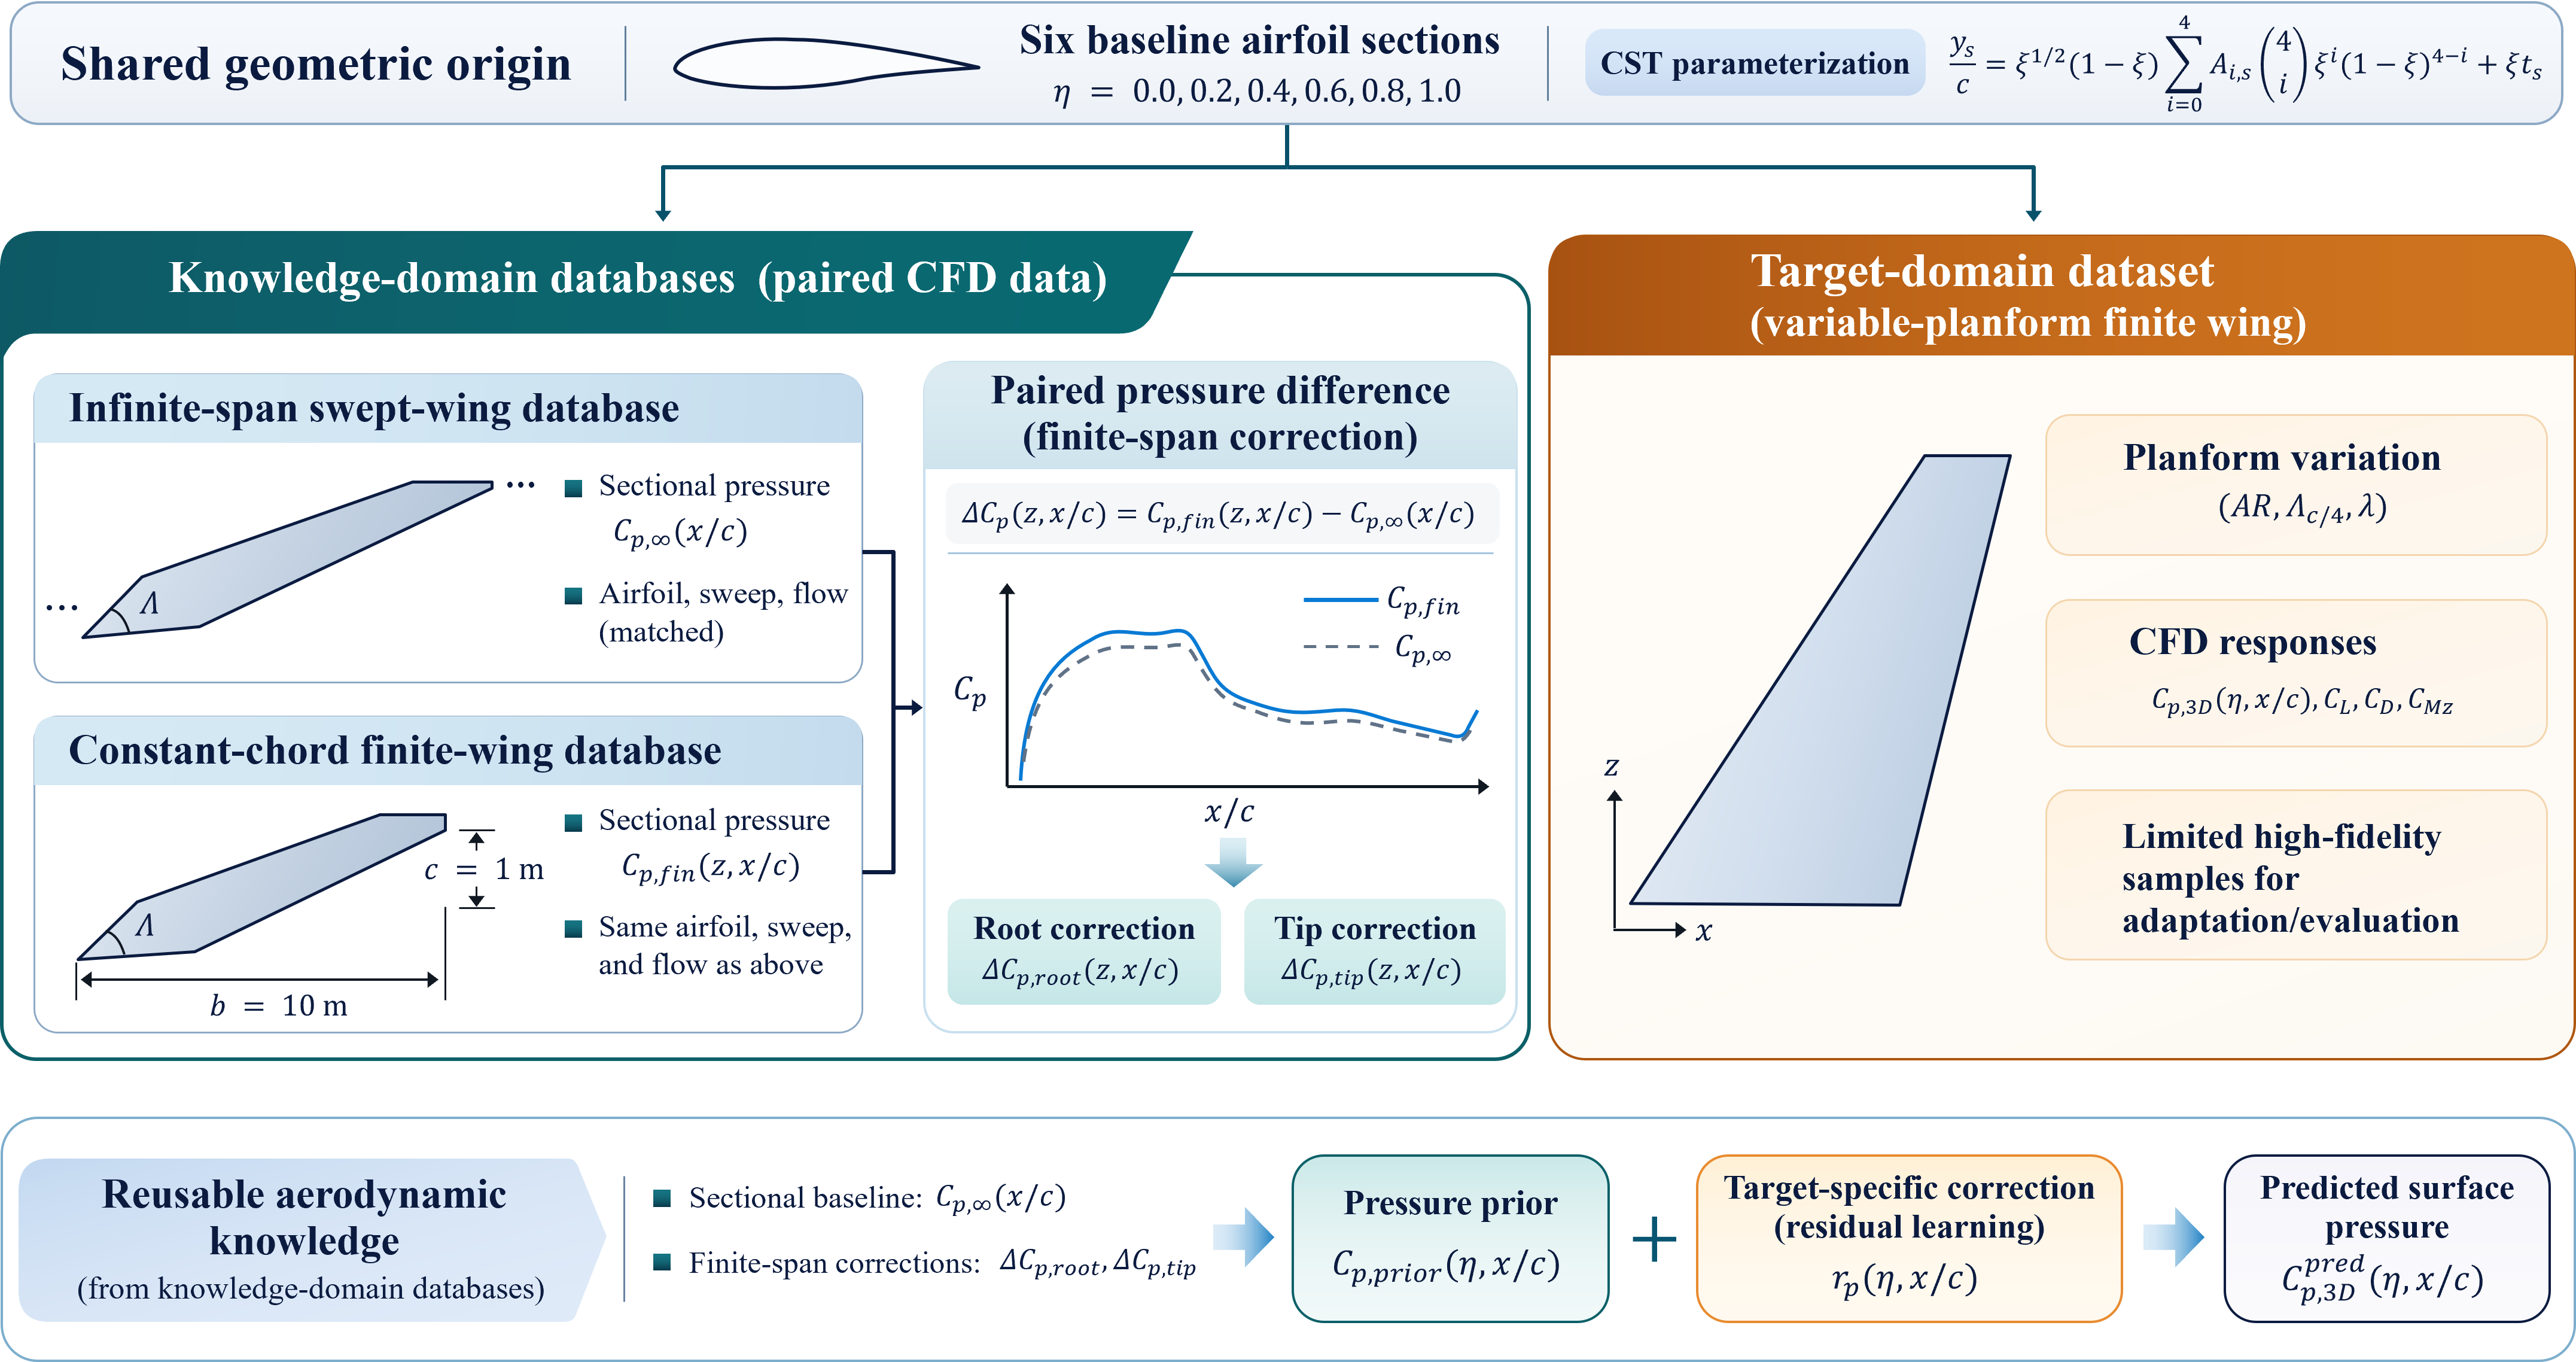
\includegraphics[width=0.98\linewidth]{II_Database_and_Preprocessing/figures/II_A_Fig03/II_A_Fig03_database_architecture.png}
    \caption{Overview of the aerodynamic databases and hierarchical knowledge transfer for finite-wing pressure prediction.}
    \label{fig:database-architecture}
\end{figure}


The infinite-span swept-wing database characterizes the baseline sectional pressure distribution $C_{p,\infty}(x/c)$ under different airfoil geometries and flow conditions. The paired constant-chord finite wings have a semispan of \SI{10}{m} and a chord of \SI{1}{m}, with the same airfoil geometry, sweep angle, and operating conditions as their infinite-span counterparts. The pressure difference associated with finite span is defined as
\begin{equation}
    \Delta C_p(z,x/c)
    = C_{p,\mathrm{fin}}(z,x/c)-C_{p,\infty}(x/c),
    \label{eq:paired-delta-cp}
\end{equation}
where $C_{p,\mathrm{fin}}(z,x/c)$ is the finite-wing sectional pressure distribution at spanwise location $z$. Because the paired calculations share the same sectional geometry and flow conditions, this difference captures the additional pressure variation associated with finite-span effects relative to the infinite-span sectional response. In view of the distinct spatial characteristics of the three-dimensional effects near the wing root and tip, the corresponding pressure differences are used separately to construct the root and tip knowledge models, denoted by $\Delta C_{p,\mathrm{root}}$ and $\Delta C_{p,\mathrm{tip}}$.

The two knowledge-domain databases share the same geometric and operating-condition sampling ranges. Five CST perturbation variables are assigned to each of the upper and lower airfoil surfaces, with normalized perturbations approximately within $[-1,1]$ and thickness-to-chord ratios primarily within $0.06$--$0.16$. The sweep angle, freestream Mach number, and angle of attack vary over $25^\circ$--$35^\circ$, $0.70$--$0.80$, and $0^\circ$--$4^\circ$, respectively, while the nominal Reynolds-number sampling range is $6.0\times10^6$--$3.0\times10^7$. The realized Reynolds numbers in the infinite-span sectional database range from approximately $5.68\times10^6$ to $3.0\times10^7$. Latin hypercube sampling (LHS) is used to sample the geometric and principal operating variables while preserving the correspondence between finite- and infinite-span cases. The two databases thus provide complementary sectional pressure and finite-span correction information for the subsequent construction of hierarchical aerodynamic priors.


\subsubsection{Target-Domain Finite-Wing Configurations and Dataset}
\label{sec:target-domain-dataset}

The two knowledge-domain databases are established independently of any specific target prediction task to extract reusable sectional aerodynamic information and regional finite-span corrections. To examine the applicability of hierarchical aerodynamic knowledge transfer with limited high-fidelity data, transonic finite wings with variable planforms are selected as a representative target domain. Compared with the constant-chord configurations used for knowledge extraction, these wings exhibit coupled variations in spanwise airfoil geometry and planform parameters, providing a setting in which to investigate the contribution of different levels of aerodynamic knowledge to three-dimensional pressure prediction.

Six spanwise airfoil sections are defined at $\eta=0.0$, $0.2$, $0.4$, $0.6$, $0.8$, and $1.0$, corresponding to the baseline stations of the reference wing. Each section is represented by five upper-surface and five lower-surface CST coefficients, yielding 60 sectional CST coefficients in total. The sectional CST coefficients are coupled through a quadratic Bernstein representation along the span, with a prescribed thickness distribution. The spanwise thickness distribution is prescribed by $t(\eta)=t_{\mathrm{tip}}+(t_{\mathrm{root}}-t_{\mathrm{tip}})(1-\eta)^p$, where $p$ controls the spanwise thickness variation.

The planform is further parameterized by aspect ratio $AR$, quarter-chord sweep angle $\Lambda_{c/4}$, and taper ratio $\lambda$, with ranges of $7.0$--$11.0$, $25^\circ$--$35^\circ$, and $0.20$--$0.40$, respectively. The root chord is fixed at \SI{5.0}{m}, and the tip chord is determined by the taper ratio. Together with freestream Mach number $M_\infty$ and angle of attack $\alpha$, varying over $0.70$--$0.80$ and $0^\circ$--$4^\circ$, respectively, the target-wing configurations are characterized by 65 parameters, comprising 60 sectional CST coefficients, three planform parameters, and two flow conditions. The principal parameters and their ranges are summarized in Table~\ref{tab:design-space}. An LHS-based sampling strategy is employed to cover the parameter space defined by the combined variations in airfoil geometry, planform, and flow conditions.

\begin{table*}[htbp]
    \centering
    \caption{Principal design variables and prescribed sampling ranges of the
    aerodynamic databases.}
    \label{tab:design-space}
    \begin{tabular}{lllll}
        \hline
        Category
        & Parameter
        & Symbol
        & Sampling range
        & Database \\
        \hline

        Operating condition
        & Mach number
        & $M_\infty$
        & $0.70$--$0.80$
        & All \\

        & Angle of attack
        & $\alpha$
        & $0^\circ$--$4^\circ$
        & All \\

        & Reynolds number
        & $Re$
        & $6.0\times10^{6}$--$3.0\times10^{7}$
        & Knowledge \\

        \hline

        Sectional geometry
        & CST perturbation
        & $\delta A_i$
        & approximately $[-1,1]$
        & All \\

        & Thickness-to-chord ratio
        & $t/c$
        & approximately $0.06$--$0.16$
        & Knowledge \\

        \hline

        Knowledge-wing geometry
        & Sweep angle
        & $\Lambda$
        & $25^\circ$--$35^\circ$
        & Knowledge \\

        & Semispan
        & $b/2$
        & \SI{10}{m}
        & Finite-wing knowledge \\

        & Chord
        & $c$
        & \SI{1}{m}
        & Finite-wing knowledge \\

        \hline

        Target-wing planform
        & Aspect ratio
        & $AR$
        & $7.0$--$11.0$
        & Target \\

        & Quarter-chord sweep angle
        & $\Lambda_{c/4}$
        & $25^\circ$--$35^\circ$
        & Target \\

        & Taper ratio
        & $\lambda$
        & $0.20$--$0.40$
        & Target \\

        & Root chord
        & $c_r$
        & \SI{5.0}{m}
        & Target \\

        \hline
    \end{tabular}
\end{table*}

The target-domain CFD data contain the three-dimensional surface-pressure distributions $C_{p,\mathrm{3D}}(\eta,x/c)$ on the upper and lower wing surfaces and the corresponding lift, drag, and pitching-moment coefficients $C_L$, $C_D$, and $C_{M_z}$. The aerodynamic coefficients are obtained directly from ADflow using the half-wing planform area and mean aerodynamic chord as the reference area and length, respectively. The pitching-moment coefficient $C_{M_z}$ is evaluated about the $z$-axis, with the moment reference point located at $(0.25c_r,0,0)$.

Independent of knowledge-domain pretraining, these high-fidelity samples are used to learn the remaining pressure discrepancy between the transferable aerodynamic prior and the target-wing response and to evaluate prediction performance with limited training data. 
